\documentclass[11pt,aspectratio=169]{beamer}

% Slide deck for the Part I compact analytical model.
% Companion source of truth: intergenerational_housing_fertility_part1.tex

\usepackage[T1]{fontenc}
\usepackage{lmodern}
\usepackage{amsmath,amssymb,mathtools}
\usepackage{booktabs}
\usepackage{tikz}
\usetikzlibrary{arrows.meta,positioning,calc,decorations.pathreplacing}
\usepackage{appendixnumberbeamer}

\setbeamertemplate{navigation symbols}{}
\setbeamertemplate{itemize items}[circle]
\setbeamertemplate{itemize subitem}{--}
\setbeamertemplate{footline}[frame number]
\setbeamersize{text margin left=0.85cm,text margin right=0.85cm}

\definecolor{accent}{RGB}{38,98,135}
\definecolor{gapred}{RGB}{160,52,42}
\definecolor{softblue}{RGB}{231,242,248}
\definecolor{softred}{RGB}{249,235,232}

\setbeamercolor{frametitle}{fg=accent}
\setbeamerfont{frametitle}{series=\bfseries,size=\large}
\setbeamercolor{title}{fg=accent}
\setbeamercolor{alerted text}{fg=gapred}
\setbeamercolor{block title}{fg=black,bg=softblue}
\setbeamercolor{block body}{fg=black,bg=softblue!45}
\linespread{1.1}

\newcommand{\dd}{\mathrm d}
\newcommand{\1}{\mathbf 1}
\newcommand{\HH}{\mathcal H}
\newcommand{\Mbar}{\bar M}

\tikzset{
  ebox/.style={draw=black!70,rounded corners=2pt,thick,align=center,inner sep=5pt,fill=white,font=\footnotesize},
  redflow/.style={-{Latex[length=2.6mm]},thick,draw=gapred},
  lab/.style={font=\scriptsize,text=black!75,align=center},
  axisline/.style={->,thick,draw=black!75}
}

\title{Intergenerational Housing Allocation and Fertility}
\subtitle{Part I: Compact Analytical Model}
\author{Tommaso De Santo}
\date{June 2026}

\begin{document}

% ============================================================
\begin{frame}
\titlepage
\vspace{-1.2em}
\begin{center}
\small
\textit{When does limited access to family-sized housing reduce fertility,\\ and which policies relax that limit?}
\end{center}
\end{frame}

% ============================================================
\begin{frame}{Overview}
\small
\textbf{Model.} Young potential parents decide whether to enter a housing market and choose tenure, housing, and completed fertility; children require goods ($\chi_i$) and housing space ($\kappa$) per child. Old incumbents choose how much owner housing to keep. Rental and owner segments offer different size menus ($\bar h^R<\bar h^O$); buying requires a down payment and payment capacity; segment prices clear aggregate markets with construction.

\medskip
\textbf{Three results.}
\begin{enumerate}\setlength{\itemsep}{0.45em}
  \item All access frictions collapse into one effective family-housing cap $H_i^m$ per household. A binding cap raises the price of a child through the space the child requires.
  \item Both markets clear, yet the allocation is inefficient when two measurable gaps are open: constrained young owners value space at $q^O+\zeta_i^{O,F}$, tax-protected old incumbents at $q^O-L_j^\tau$.
  \item The fertility effect of a policy is a transparent local formula: exposure $\times$ pass-through to the cap $\times$ fertility response, plus entry, plus a tenure-switching margin whose sign depends on which tenure is the expensive way to occupy space.
\end{enumerate}
\end{frame}

% ============================================================
\begin{frame}{Young households}
\small
Type $i=(y_i,a_i,B_i)\sim G_Y$: income, liquid wealth, inheritance exposure. Wealth is pledgeable only,
\[
A_i(x)=a_i+xB_i+T_i^b(x),
\qquad x=1-\tau^b,
\]
backing down payments but not entering the flow budget.

\medskip
Children require goods and space; parents consume the residual:
\[
c_i=C_i-\chi_i n_i,
\qquad
s_i=h_i-\kappa n_i,
\qquad
u_i^Y=\log c_i+\alpha\log s_i+\beta\log n_i .
\]
Substituting $h=s+\kappa n$ into a branch budget with user cost $q^m$:
\[
c_i+q^m s_i+\underbrace{(\chi_i+\kappa q^m)}_{\text{full price of a child}}n_i=y_i .
\]
\smallskip
Unconstrained, a child costs its goods plus its space at the \emph{market} price. Under binding constraints the space term will carry a premium --- that is the transmission channel. ($\beta\log n_i$ rules out $n_i=0$: intensive margin only.)
\end{frame}

% ============================================================
\begin{frame}{Tenure branches and the effective family-housing cap}
\small
Conditional on entry, households solve a renter and an owner branch and take the better one, $W_i^Y=\max\{W_i^R,W_i^O\}$:
\[
W_i^m=\max_{c,h,n}\;u_i^Y(c,h,n)
\quad\text{s.t.}\quad
c+q^m h+\chi_i n=y_i,\;\; h\le H_i^m,
\]
where all access constraints collapse into one cap per branch:
\[
H_i^R=\bar h^R,
\qquad
H_i^O=\min\Big\{
\underbrace{\bar h^O}_{\text{menu}},\;
\underbrace{\tfrac{A_i(x)\,\rho_p}{(1-\phi)\,q^O}}_{\text{down payment}},\;
\underbrace{\tfrac{\psi y_i}{q^O}}_{\text{payment-to-income}}
\Big\},
\qquad
\rho_p=r+\delta^O+\tau^p .
\]
\smallskip
A renter is capped by the stock; a buyer by whichever of menu, collateral, or debt service is shortest. Policy moves fertility only through the \emph{binding} component of $H_i^m$.

\smallskip
\footnotesize Note: $P^O=q^O/\rho_p$ enters only the down payment, so a higher property tax \emph{relaxes} the collateral constraint.
\end{frame}

% ============================================================
\begin{frame}{Entry and old households}
\small
\textbf{Entry.} Logit over inside value vs.\ outside option $\bar W^E$ (taste-shock scale $\kappa_E$):
\[
\pi_i^E=\frac{\exp\{W_i^Y/\kappa_E\}}{\exp\{W_i^Y/\kappa_E\}+\exp\{\bar W^E/\kappa_E\}} .
\]

\medskip
\textbf{Old incumbents.} Endowment $H_j^0$; choose consumption, retained housing, bequests:
\[
\max\;\log c_j^O+\gamma\log h_j^O+\mathcal B_j(e_j)
\quad\text{s.t.}\quad
c_j^O+e_j+(q^O-L_j^\tau)h_j^O=m_j+q^OH_j^0,
\quad 0\le h_j^O\le H_j^0,
\]
where $L_j^\tau=\tau^pP^O-\tilde\tau_j\tilde P_j\ge0$ is the incumbent assessment discount: market tax cost minus protected tax cost.

\medskip
Releasing a unit earns $q^O$; keeping it costs $q^O-L_j^\tau$. The discount is a \alert{subsidy to staying put} --- a tax rule, not a preference. Bequests $\mathcal B_j$ are a preference and are respected throughout.
\end{frame}

% ============================================================
\begin{frame}{Competitive equilibrium}
\small
Prices $(q^R,q^O)$, asset price $P^O=q^O/\rho_p$, construction $(I^R,I^O)$ such that:
\begin{itemize}\setlength{\itemsep}{0.3em}
  \item households optimize: branch problems, tenure choice, logit entry; old retention;
  \item competitive construction: $q^m=\Phi_I^m(I^m;Z^m)$ (flow units);
  \item both segments clear in aggregate:
  \[
  \Mbar\!\int\!\pi_i^E\1\{o_i{=}R\}h_i\,\dd G_Y=\bar H^R+I^R,
  \qquad
  \Mbar\!\int\!\pi_i^E\1\{o_i{=}O\}h_i\,\dd G_Y+\!\int\! h_j^O\,\dd F_O=\bar H^O+I^O;
  \]
  \item housing payments are transfers closed by lump-sum rebates; only construction uses real resources.
\end{itemize}
\medskip
Clearing pins aggregates, not assignment: nothing in these conditions asks whether the marginal family-sized unit is held by the household that values it most.
\end{frame}

% ============================================================
\begin{frame}{Marginal values and access gaps}
\small
A constrained household values space above its price; the gap is the constraint's bite, in goods, read off the bundle:
\[
MV_i^m=\frac{\alpha c_i^m}{s_i^m}=q^m+\zeta_i^m,
\qquad
\zeta_i^m=\frac{\alpha c_i^m}{s_i^m}-q^m\ge0 .
\]
For owners the gap decomposes by the constraint that generates it:
\[
\zeta_i^O
=
\underbrace{\frac{\mu_i}{\lambda_i^O}(1-\phi)P^O}_{\text{collateral}}
+
\underbrace{\frac{\eta_i}{\lambda_i^O}q^O}_{\text{debt service}}
+
\underbrace{\frac{\theta_i^O}{\lambda_i^O}}_{\text{menu}}
\;=\;
\zeta_i^{O,F}+\text{menu part}.
\]
\begin{block}{Proposition 1 (fertility condition)}
\centering
$\displaystyle \frac{\beta c_i^m}{n_i^m}=\chi_i+\kappa\big(q^m+\zeta_i^m\big)$
\end{block}
\smallskip
A child's space is priced at the household's \emph{own} shadow value of space: children get more expensive exactly where family-sized space is hard to reach, at unchanged market prices.
\end{frame}

% ============================================================
\begin{frame}{Two gaps separate the equilibrium from the planner}
\footnotesize
Planner: same preferences, same menus, same construction technology; financial (DP/PTI) constraints relaxable at zero marginal resource cost; fertility-neutral; entry and tenure assignments held at equilibrium.
\begin{center}
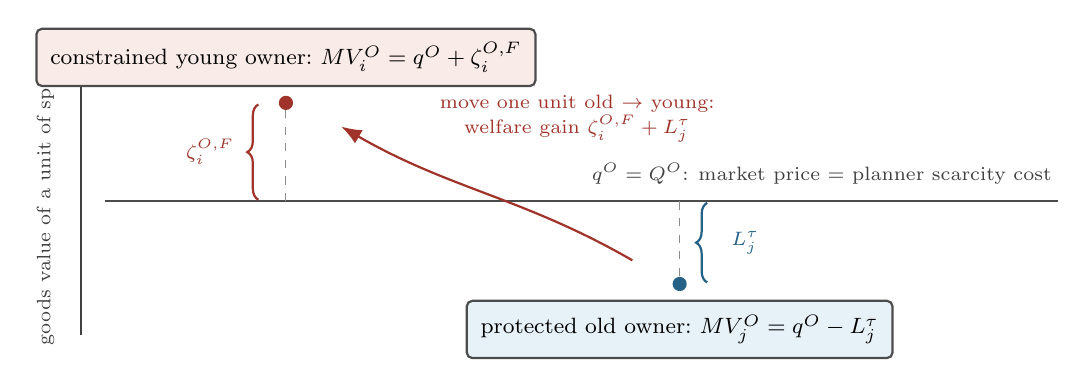
\begin{tikzpicture}[x=1cm,y=1cm]
  \draw[axisline] (0,-1.7) -- (0,1.6);
  \node[lab,rotate=90,anchor=south] at (-0.22,0) {goods value of a unit of space};
  \draw[thick,black!70] (0.3,0) -- (12.4,0);
  \node[lab,anchor=south east] at (12.45,0.09) {$q^O=Q^O$: market price $=$ planner scarcity cost};
  \fill[gapred] (2.6,1.25) circle (0.09);
  \node[ebox,fill=softred,anchor=south] at (2.6,1.45) {constrained young owner:\ $MV_i^O=q^O+\zeta_i^{O,F}$};
  \draw[decorate,decoration={brace,amplitude=4pt},thick,gapred] (2.25,0.02) -- (2.25,1.23) node[midway,left=5pt,lab,text=gapred]{$\zeta_i^{O,F}$};
  \draw[black!45,dashed] (2.6,0) -- (2.6,1.25);
  \fill[accent] (7.6,-1.05) circle (0.09);
  \node[ebox,fill=softblue,anchor=north] at (7.6,-1.25) {protected old owner:\ $MV_j^O=q^O-L_j^\tau$};
  \draw[decorate,decoration={brace,amplitude=4pt},thick,accent] (7.95,-1.03) -- (7.95,-0.02) node[midway,right=5pt,lab,text=accent]{$L_j^\tau$};
  \draw[black!45,dashed] (7.6,0) -- (7.6,-1.05);
  \draw[redflow] (7.0,-0.75) to[out=150,in=-30] (3.3,0.95);
  \node[lab,text=gapred] at (6.3,1.05) {move one unit old $\to$ young:\\ welfare gain $\zeta_i^{O,F}+L_j^\tau$};
\end{tikzpicture}
\end{center}
\vspace{0.1em}
The equilibrium satisfies the planner's marginal conditions \textbf{only if} $\zeta_i^{O,F}=0$ and $L_j^\tau=0$. Binding size \emph{menus} are not a gap (the planner faces the same stock); old occupancy per se is not a gap (true utility and bequests are counted).
\end{frame}

% ============================================================
\begin{frame}{Fertility and the family-housing cap}
\begin{columns}[T]
\begin{column}{0.50\textwidth}
\begin{center}
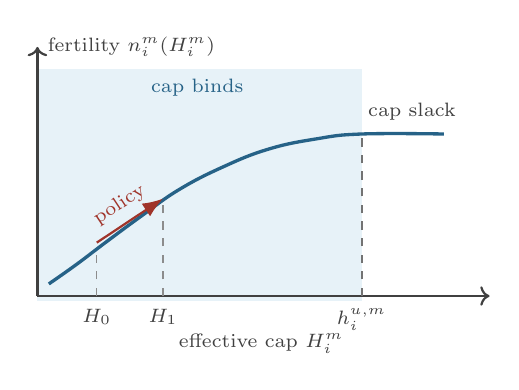
\begin{tikzpicture}[x=0.58cm,y=0.57cm]
  \fill[softblue] (0.7,0.45) rectangle (7.8,5.6);
  \node[lab,text=accent] at (4.2,5.2) {cap binds};
  \draw[axisline] (0.7,0.55) -- (10.6,0.55);
  \node[lab] at (5.6,-0.5) {effective cap $H_i^m$};
  \draw[axisline] (0.7,0.55) -- (0.7,6.1) node[right,lab]{fertility $n_i^m(H_i^m)$};
  \draw[very thick,draw=accent]
    plot[smooth,tension=0.72] coordinates {
      (0.95,0.82) (1.55,1.25) (2.2,1.75) (3.0,2.35)
      (3.8,2.92) (4.75,3.42) (5.75,3.82) (6.8,4.05)
      (7.8,4.16) (9.6,4.16)
    };
  \draw[dashed,thick,draw=black!55] (7.8,0.55) -- (7.8,4.16);
  \node[lab,below] at (7.8,0.48) {$h_i^{u,m}$};
  \node[lab,above] at (8.9,4.25) {cap slack};
  \draw[dashed,draw=black!45] (2.0,0.55) -- (2.0,1.62);
  \node[lab,below] at (2.0,0.48) {$H_0$};
  \draw[dashed,draw=black!45] (3.45,0.55) -- (3.45,2.7);
  \node[lab,below] at (3.45,0.48) {$H_1$};
  \draw[redflow] (2.0,1.74) -- (3.45,2.72) node[midway,above,sloped,lab,text=gapred]{policy};
\end{tikzpicture}
\end{center}
\end{column}
\begin{column}{0.47\textwidth}
\small
With a binding cap, $h=H$ and
\[
\frac{\dd n}{\dd H}
=
\frac{\dfrac{\alpha\kappa}{s^2}-\dfrac{\chi q}{c^2}}
{\dfrac{\beta}{n^2}+\dfrac{\chi^2}{c^2}+\dfrac{\alpha\kappa^2}{s^2}} .
\]
\begin{itemize}\setlength{\itemsep}{0.35em}
  \item More space lowers the crowding cost of a child; but the household also buys more housing, squeezing consumption.
  \item Fertility rises at every binding cap iff
  $\chi\le\kappa q^m/\alpha$: children no more goods-intensive than their parents' bundle (one curve per branch).
\end{itemize}
\end{column}
\end{columns}
\end{frame}

% ============================================================
\begin{frame}{Equal scaling: the access gap predicts the fertility response}
\small
Define the within-branch response $\Psi_i^m=\partial n_i^m/\partial H_i^m$ at a binding cap. Under equal scaling,
\[
\Psi_i^m
=
\frac{\kappa}{\alpha}\,
\frac{\zeta_i^m}{c_i^m}\,
\Omega_i^m,
\qquad
\Omega_i^m=
\frac{\dfrac{\alpha}{s_i^m}+\dfrac{q^m}{c_i^m}}
{\dfrac{\beta}{(n_i^m)^2}+\dfrac{\chi_i^2}{(c_i^m)^2}+\dfrac{\alpha\kappa^2}{(s_i^m)^2}}
>0 .
\]
\begin{itemize}\setlength{\itemsep}{0.4em}
  \item $\Psi_i^m>0$ iff $\zeta_i^m>0$: fertility responds exactly for the households whose constraint bites, more where it bites harder.
  \item The entry margin runs on the same object: relaxing the cap raises inside value by $\Theta_i^m=\lambda_i^m\zeta_i^m=\zeta_i^m/c_i^m$ per unit.
  \item The gap that measures misallocation is the gap that predicts births.
\end{itemize}
\end{frame}

% ============================================================
\begin{frame}{A local policy decomposition}
\small
Let $P_i^m(z)=\partial H_i^m/\partial z$ (pass-through to the cap) and $\mathcal B_m$ the entrant types whose cap binds in branch $m$. Holding prices, tenure, and active sets fixed:
{\footnotesize
\[
\left.\frac{\dd N}{\dd z}\right|_{q,o,\mathcal A}
=
\Mbar\sum_{m\in\{R,O\}}\int_{\mathcal B_m}
\Bigg[
\underbrace{\pi_i^E\,\Psi_i^m}_{\substack{\text{intensive margin}}}
+
\underbrace{(n_i^m-\bar n_i^E)\,\frac{\pi_i^E(1-\pi_i^E)}{\kappa_E}\,\Theta_i^m}_{\substack{\text{entry margin}}}
\Bigg]
\underbrace{P_i^m(z)}_{\substack{\text{pass-through}}}
\,\dd G_Y(i)
\]}
\begin{itemize}\setlength{\itemsep}{0.35em}
  \item Exposure $\times$ pass-through $\times$ response, plus entry (births net of outside-option fertility $\bar n_i^E$).
  \item The cap is a minimum: a policy that improves a slack component has $P_i^m=0$ --- no effect through this channel. Price-type policies are outside the fixed-price formula.
  \item Left out: price/construction responses, fiscal costs $\Xi^\Pi$ (general equilibrium) --- and tenure switching, which is first order at fixed prices. Next slide.
\end{itemize}
\end{frame}

% ============================================================
\begin{frame}{Tenure switching at the boundary}
\small
Tenure is discrete, so switchers' bundles---and fertility---jump at $W_i^R=W_i^O$. The size of the margin is quantitative; the sign is theory.

\begin{block}{Proposition (fertility at a tenure switch)}
At indifference between a cheap branch ($q^A$) and an expensive branch ($q^B>q^A$): the cheap branch's cap binds, and the expensive branch has more housing, more slack space, less consumption. If $\chi\le\kappa q^A/\alpha$, it also has higher fertility: $n_B>n_A$.
\end{block}
The only reason to pay more per unit of space is to get more space; space-intensive children come with it. Three rent/own cases:
\begin{itemize}\setlength{\itemsep}{0.3em}
  \item $q^O>q^R$: switchers into ownership upsize, $n_O>n_R$ --- switching term $\ge0$; the fixed-tenure formula is a \textbf{lower bound} for owner-access policies.
  \item $q^O=q^R$: allocations continuous at the boundary, no jump --- the formula is \textbf{exact}.
  \item $q^O<q^R$: switchers downsize into cheaper owned units, $n_O<n_R$ --- switching term $\le0$; an \textbf{upper bound}. Which case applies is one benchmark number: owner user cost vs.\ rent per unit.
\end{itemize}
\end{frame}

% ============================================================
\begin{frame}{Which policies move fertility through this channel}
\small
\begin{columns}[T]
\begin{column}{0.50\textwidth}
\textbf{Pass (when the named component binds)}
\footnotesize
\begin{itemize}\setlength{\itemsep}{0.35em}
  \item Down-payment grants, LTV relief ($A_i$, $\phi$): $P_i^O=\rho_p/[(1-\phi)q^O]$ when collateral binds.
  \item Payment-to-income relaxation ($\psi$): $P_i^O=y_i/q^O$ when debt service binds.
  \item Family-sized rental supply or conversion ($\bar h^R$): $P_i^R=1$ for menu-capped renters.
  \item Assessment reform: shrinks $L_j^\tau$, releases old-held space.
\end{itemize}
\end{column}
\begin{column}{0.47\textwidth}
\textbf{No effect through this channel}
\footnotesize
\begin{itemize}\setlength{\itemsep}{0.35em}
  \item Subsidies to units below the binding size: the binding component does not move.
  \item Price subsidies that leave $H_i^m$ unchanged: real effects, but they require the GE analysis.
  \item Liquidity to households with slack constraints: pledgeable wealth has no income effect.
\end{itemize}
\smallskip
\textbf{Property tax is two-sided}: the level relaxes young down payments (lower $P^O$); assessment \emph{protection} is what creates old lock-in.
\end{column}
\end{columns}
\end{frame}

% ============================================================
\begin{frame}{Takeaways}
\begin{enumerate}\setlength{\itemsep}{0.9em}
  \item \textbf{Family-housing access is a fertility margin.} Children are priced at the household's own shadow value of space, $\beta c_i/n_i=\chi_i+\kappa(q^m+\zeta_i^m)$; under $\chi_i\le\kappa q^m/\alpha$, relaxing a binding cap raises fertility.
  \item \textbf{Two measurable gaps separate equilibrium from the planner}: the young financing gap $\zeta_i^{O,F}$ and the old assessment discount $L_j^\tau$. Reallocating one unit old $\to$ young is worth $\zeta_i^{O,F}+L_j^\tau$. The young mechanism stands without the old one.
  \item \textbf{Policy works only through the binding component of $H_i^m$.} Local effect $=$ exposure $\times$ pass-through $\times$ response $+$ entry; under equal scaling $\Psi_i^m\propto\zeta_i^m$. Tenure switching reinforces owner-access policies when ownership is the expensive family-space segment, and vanishes at price parity.
\end{enumerate}
\end{frame}

% ============================================================
\appendix

\begin{frame}{Appendix: the branch derivative}
\small
If $0<H<h^u$, the cap binds, $h(H)=H$, and
\[
c(H)=y-qH-\chi n(H),
\qquad
s(H)=H-\kappa n(H).
\]
Fertility solves $F(n,H)=\dfrac{\beta}{n}-\dfrac{\chi}{c(H)}-\dfrac{\alpha\kappa}{s(H)}=0$, and
\[
F_n=-\Big[\frac{\beta}{n^2}+\frac{\chi^2}{c^2}+\frac{\alpha\kappa^2}{s^2}\Big]<0,
\qquad
F_H=\frac{\alpha\kappa}{s^2}-\frac{\chi q}{c^2},
\qquad
\frac{\dd n}{\dd H}=-\frac{F_H}{F_n}.
\]
Unconstrained benchmark (Cobb--Douglas in $(c,s,n)$ at prices $(1,q,\chi+\kappa q)$):
\[
c^u=\frac{y}{1+\alpha+\beta},
\qquad
n^u=\frac{\beta y}{(1+\alpha+\beta)(\chi+\kappa q)},
\qquad
\frac{q s^u}{c^u}=\alpha .
\]
\end{frame}

\begin{frame}{Appendix: equal scaling and the access gap}
\small
At a binding cap, $\alpha c_i^m/s_i^m=q^m+\zeta_i^m$. Under equal scaling $\chi_i=\kappa q^m/\alpha$, the numerator of $\Psi_i^m$ factors:
\[
\frac{\alpha\kappa}{(s_i^m)^2}-\frac{\chi_i q^m}{(c_i^m)^2}
=
\frac{\kappa}{\alpha}
\Big(\frac{\alpha}{s_i^m}-\frac{q^m}{c_i^m}\Big)
\Big(\frac{\alpha}{s_i^m}+\frac{q^m}{c_i^m}\Big),
\qquad
\frac{\alpha}{s_i^m}-\frac{q^m}{c_i^m}=\frac{\zeta_i^m}{c_i^m},
\]
so $\Psi_i^m=\frac{\kappa}{\alpha}\,\frac{\zeta_i^m}{c_i^m}\,\Omega_i^m$ with $\Omega_i^m>0$.
The envelope value of relaxing the cap is $\Theta_i^m=\partial W_i^m/\partial H_i^m=\lambda_i^m\zeta_i^m$ with $\lambda_i^m=1/c_i^m$, and the logit entry response is $\partial\pi_i^E/\partial W_i^Y=\pi_i^E(1-\pi_i^E)/\kappa_E$.
\end{frame}

\begin{frame}{Appendix: planner conditions and the comparison}
\small
With goods multiplier $\Lambda$ and segment multipliers $\Lambda Q^m$, interior planner allocations satisfy, away from menu corners,
\[
\frac{u_{h,i}^Y}{u_{c,i}^Y}=Q^{m},
\qquad
\frac{u_{h,j}^O}{u_{c,j}^O}=Q^O,
\qquad
Q^m=\Phi_I^m(I^m;Z^m),
\qquad
\frac{\beta c_i}{n_i}+\nu_i^g=\chi_i+\kappa Q^{o_i^P}.
\]
Endogenous logit entry enters all allocation FOCs through a common factor that cancels from these ratios.

\medskip
At an interior competitive allocation, clearing and competitive construction give $Q^R=q^R$, $Q^O=q^O$, and competitive marginal values are
\[
MV_i^R=q^R+\zeta_i^R,
\qquad
MV_i^O=q^O+\zeta_i^O,
\qquad
MV_j^O=q^O-L_j^\tau .
\]
If DP/PTI are relaxable at zero marginal resource cost, the CE satisfies the planner's conditional FOCs only if $\zeta_i^{O,F}=0$ and $L_j^\tau=0$; menus common to both problems generate no gap. Entry and tenure-assignment efficiency are not characterized.
\end{frame}

\begin{frame}{Appendix: accounting conventions}
\small
\begin{itemize}\setlength{\itemsep}{0.45em}
  \item \textbf{Flow normalization.} $q^m$ is both the user cost and the marginal resource cost of segment-$m$ services; $\Phi^m$ is in flow units, so $q^m=\Phi_I^m$. $P^O$ only converts $q^O$ into the purchase price for down payments. (Under asset-unit costs, $P^O=\Phi_I^O$ and the property tax would also distort construction.)
  \item \textbf{Stocks.} $\int H_j^0\,\dd F_O+H_{\mathrm{pass}}^O=\bar H^O$; rental stock held by passive landlords; passive and fiscal income rebated lump-sum.
  \item \textbf{Bequest loop is open (reduced form).} Old bequest expenditure $e_j$ is a current resource use; young exposure $B_i$ is a primitive of $G_Y$. The estate tax $\tau^b$ works only through pledgeable resources $A_i(x)$.
  \item \textbf{Outside fertility.} $N$ counts births among entrants; with outside births $\bar n_i^E$, entry-margin terms use $n_i^Y-\bar n_i^E$.
\end{itemize}
\end{frame}

\end{document}
